\documentclass[10pt,crop]{standalone}
\usepackage{tikz}
\usetikzlibrary{backgrounds,calc,positioning}
\begin{document}
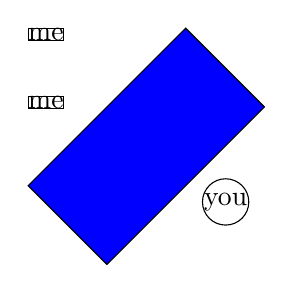
\begin{tikzpicture}{tight background,background rectangle/.style={fill=green},show background rectangle,}
  \path[draw=black,fill=blue,use as bounding box] (0,-1) -- (-1,0) -- (1,2) -- (2,1) --cycle;
  \node[draw,rectangle,inner sep=0pt,anchor=north west] at (current bounding box.north west)(me){me};
  \node[draw,rectangle,inner sep=0pt,anchor=north west,below=.7cm of me] {me};
  \node[draw,circle,inner sep=0pt,anchor=south] at ($(current bounding box.south east) + (-.5,.5)$) {you};
\end{tikzpicture}
\end{document}
